%!TEX root = ../slides.tex
\section{Solution}
{\aauwavesbg%
\begin{frame}[plain]
  \begin{textblock*}{8.5cm}(4.3cm,8.3cm)
  \small
  \textbf{Architecture of proposed system solution. The global perception-action cycle, the different memory types, and the internal feedback loops are observed.}
  \end{textblock*}

  \begin{textblock*}{1cm}(12cm,9.3cm)
  \scriptsize
  \insertframenumber~/~\inserttotalframenumber
  \end{textblock*}

  \centering
  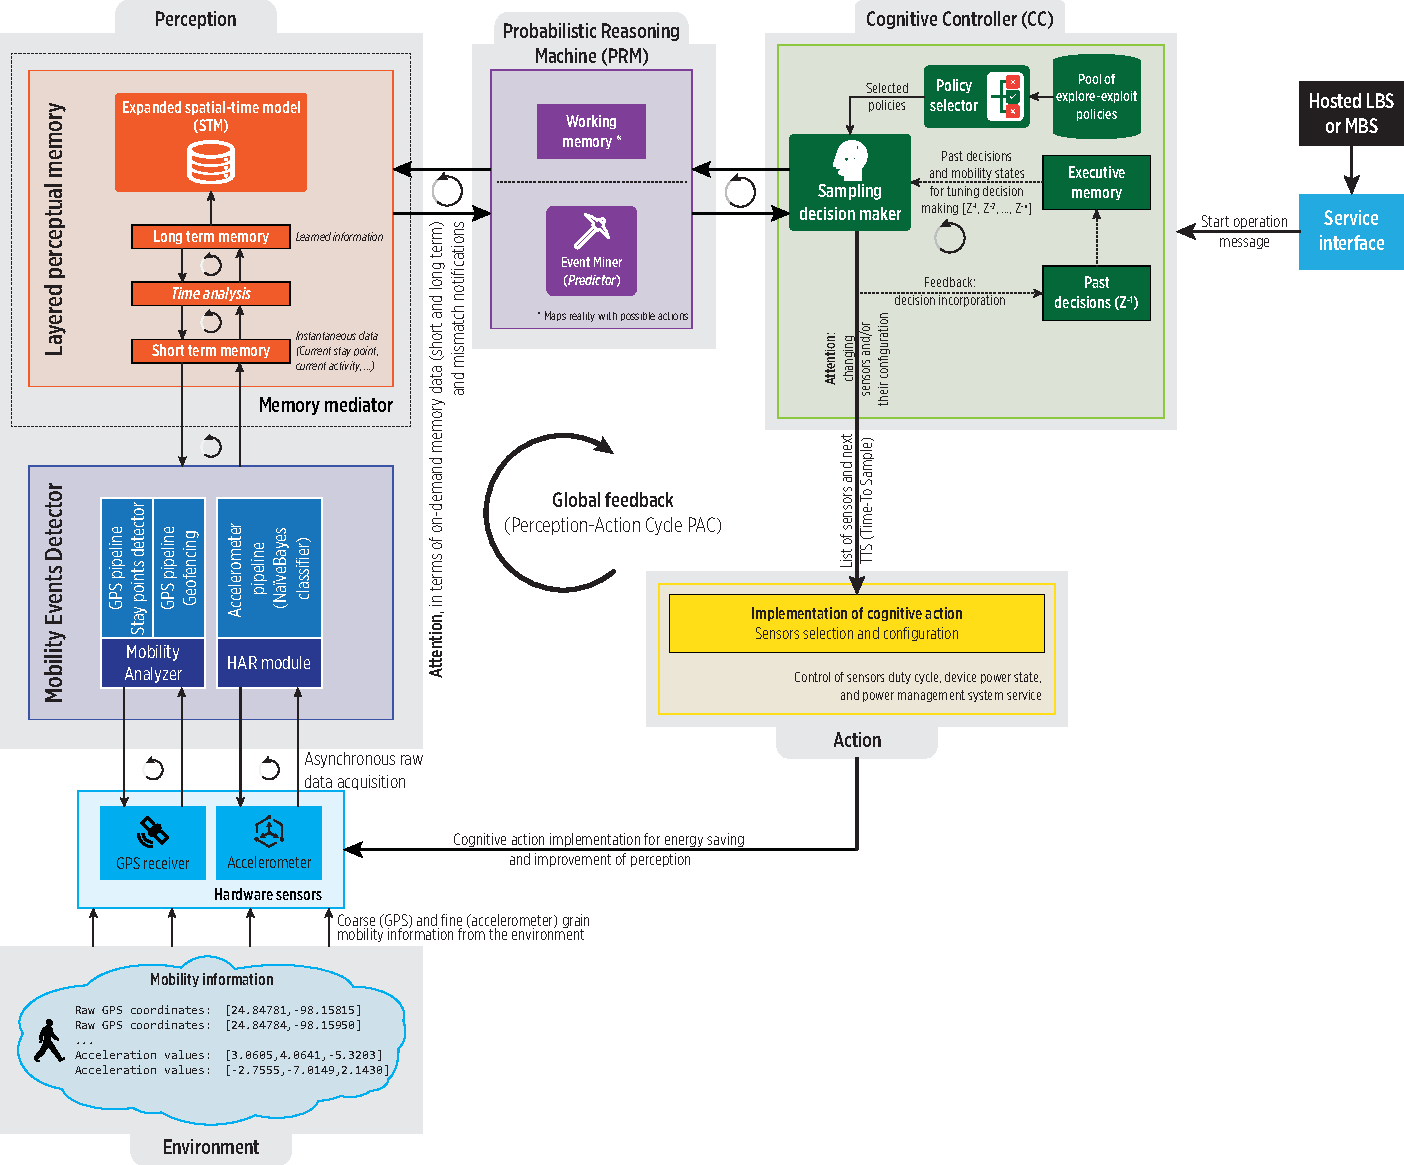
\includegraphics[width=0.98\textwidth]{vectors/inspired-cds-solution-for-slides}
\end{frame}}
    

\subsection{Perception components}
\begin{frame}{Perception components}{Mobility Events Detector}
\small
\begin{figure}
    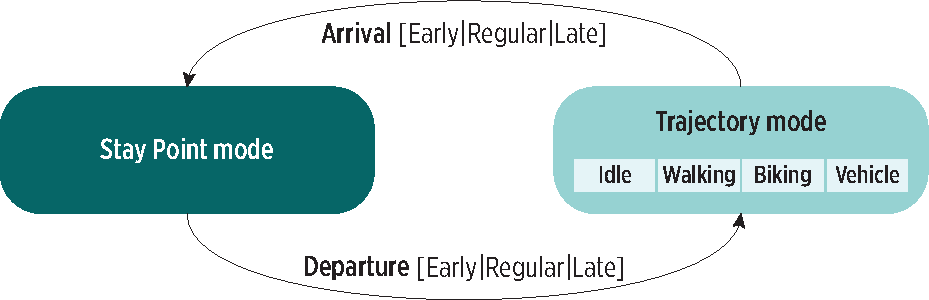
\includegraphics[width=0.55\textwidth]{vectors/mobility-as-events}
    \caption{Individual's mobility as a sequence of high level states and associated events detected from raw sensor data~\cite{Alessandretti2017,Wang2014}.}
\end{figure}

\begin{block}{\small \textbf{Mobility Events Detector}} 
Aime at identifying:
\begin{itemize}
    \item Coarse-grain mobility events.
    \item Fine-grain mobility events.
\end{itemize}
\end{block}
\end{frame}

\begin{frame}{Perception components}{Mobility Events Detector: \emph{Stay Points Detector} module}
\small
\begin{columns}
\begin{column}[T]{0.5\textwidth}
\begin{block}{\small \emph{\textbf{Stay Points Detector}} module}
\begin{itemize}
    \item Focused on detecting stay points in user mobility.
    \item Event driven design, it incrementally processes each low-level mobility event (raw GPS data).
\end{itemize}
\begin{figure}
  \centering
  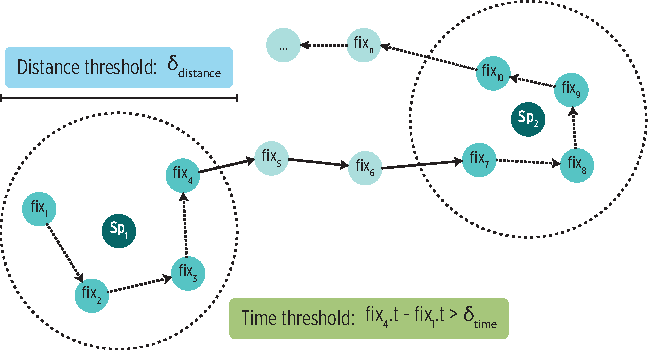
\includegraphics[width=0.9\textwidth]{vectors/zhen-algorithm-behavior}
  \caption{A conceptual representation of the stay points detection algorithm behavior.}
\end{figure}
\end{block}
\end{column}

\begin{column}[T]{0.5\textwidth}
\begin{block}{\small \emph{\textbf{Geofencing}} module}
\begin{itemize}
    \item Window-based approach with voting system.
    \item Requires an $SPS_{candidate}$ list of stay points.
    \item Incrementally analyzes GPS fixes for detecting coarse- grain mobility events under a $gf_{distance}$ threshold:
\end{itemize}

\begin{figure}
  \centering
  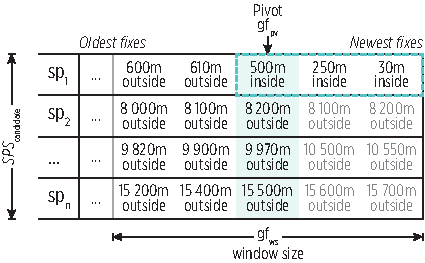
\includegraphics[width=0.75\textwidth]{vectors/geofencing-window-based-snapshot-for-slides}
  \caption{A conceptual representation of the window-based geofencing operation.}
\end{figure}
\end{block}
\end{column}
\end{columns}


\end{frame}

% \begin{frame}{Perception components}{Mobility Events Detector: \emph{Geofencing} module}
% \small
% \vspace{-0.3cm}
% \begin{block}{\small \emph{\textbf{Geofencing}} module}
% \begin{itemize}
%     \item Window-based approach with voting system.
%     \item Requires an $SPS_{candidate}$ list of stay points.
%     \item Incrementally analyzes location fixes for detecting coarse-grain mobility events under a $gf_{distance}$ threshold:
% \end{itemize}

% {
% \centering
% \resizebox{0.65\textwidth}{!}{%
% \begin{tabular}{@{}llll@{}}
% \toprule
% \multicolumn{1}{c}{\textbf{Older fixes window}} & \multicolumn{1}{c}{\textbf{Pivot ($gf_{pv}$)}} & \multicolumn{1}{c}{\textbf{Newer fixes window}} & \multicolumn{1}{c}{\textbf{Outcome}} \\ \midrule
% outside & inside & inside & $arrival = ( sp, t_{in} )$ \\
% inside & outside & outside & $departure = (sp, t_{out})$ \\
% inside & inside & inside & $no\_change_{sp} = (sp, t)$ \\  
% outside & outside & outside & $no\_change_{trj} = (none, t)$ \\ \bottomrule
% \end{tabular}%
% }
% \par 
% }
% \end{block}

% \begin{figure}
%   \centering
%   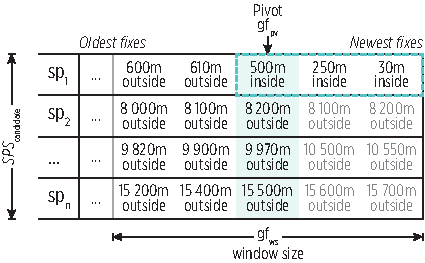
\includegraphics[width=0.47\textwidth]{vectors/geofencing-window-based-snapshot-for-slides}
%   \caption{A conceptual representation of the window-based geofencing operation.}
%   \label{fig:geofencing-window-based-snapshot}
% \end{figure}
% \end{frame}

\begin{frame}{Perception components}{Mobility Events Detector: \emph{HAR} module}
\small
\begin{block}{\small \emph{\textbf{HAR}} module}
\begin{itemize}
    \item Window-based approach.
    \item Detects transportation mode from accelerometer data.
    \item Underlying NaïveBayes classifier.
\end{itemize}
\end{block}

\begin{figure}
  \centering
  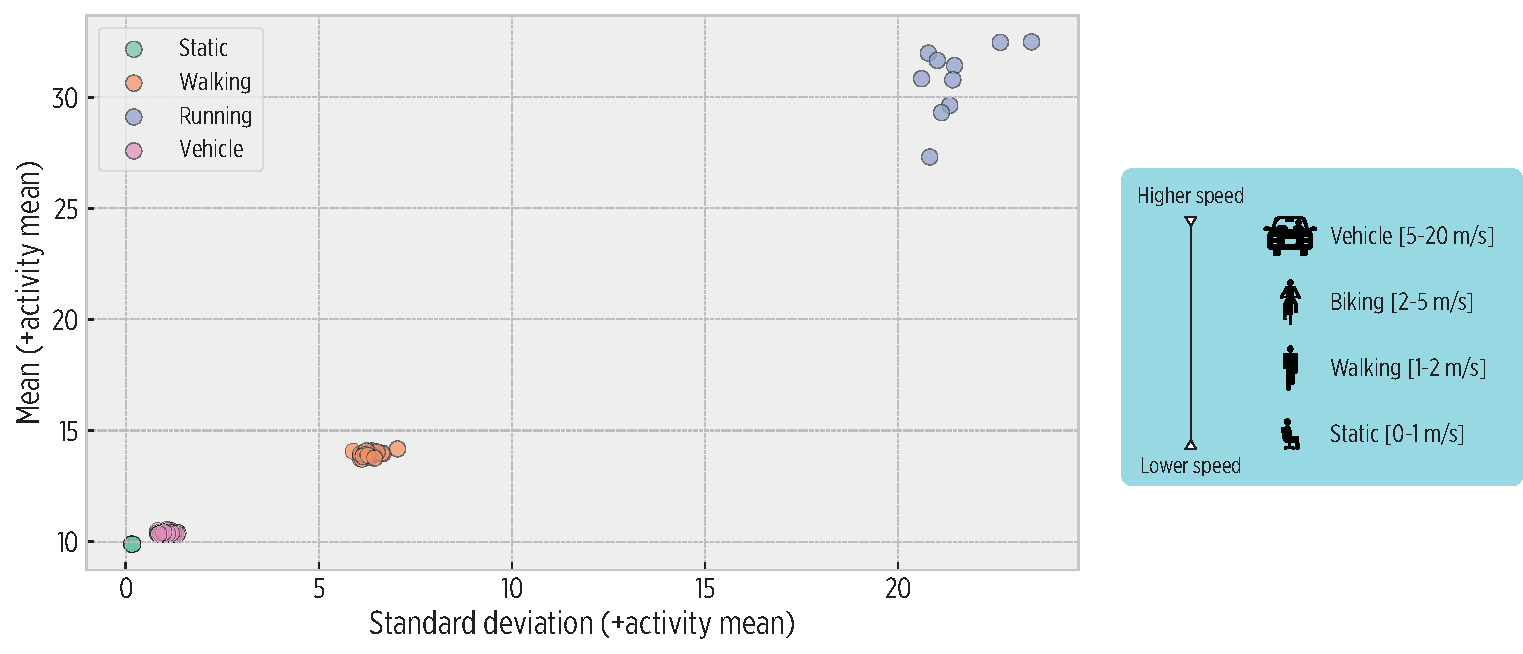
\includegraphics[width=0.9\textwidth]{vectors/har-patterns-for-slides-v2}
  \caption{Distribution of mean and standard deviation features employed by the NaïveBayes classifier of the HAR module.}
\end{figure}
\end{frame}

% \subsection{Layered perceptual memory}
\begin{frame}{Layered perceptual memory}{Short and long-term memory information}
\vspace{-0.25cm}
\small
\begin{block}{\small \textbf{Layered perceptual memory}}
\begin{itemize}
    \item Short-term memory information: current (observed) mobility status.
    \item Long-term memory information: the Expanded Spatial-Time model (STM).
\end{itemize}
\end{block}

\begin{block}{\small \textbf{Expanded Spatial-Time model}}
\begin{itemize}
  \item The highest level of mobility information held by the system.
\end{itemize}
{
  \centering
  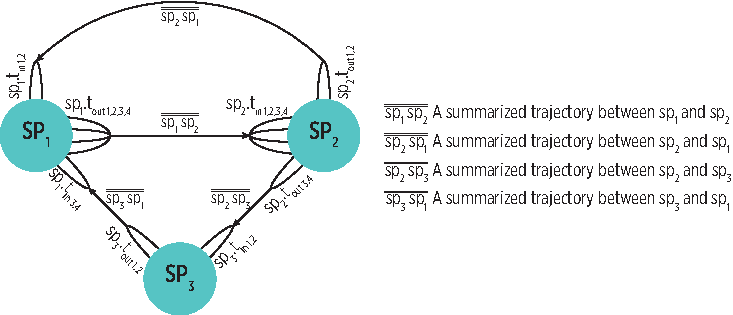
\includegraphics[width=0.7\textwidth]{vectors/stm-slides}
  \captionof{figure}{A conceptual representation of the STM's structure.}
\par }
\end{block}
\end{frame}

\begin{frame}{Layered perceptual memory}{Expanded Spatial-Time model (STM)}
\small
\begin{block}{\small \textbf{Generation of the STM}}
\begin{itemize}
    \item Incrementally built with the coarse-grain mobility events detected by the \emph{Mobility Events Detector}.
\end{itemize}
{
  \centering
  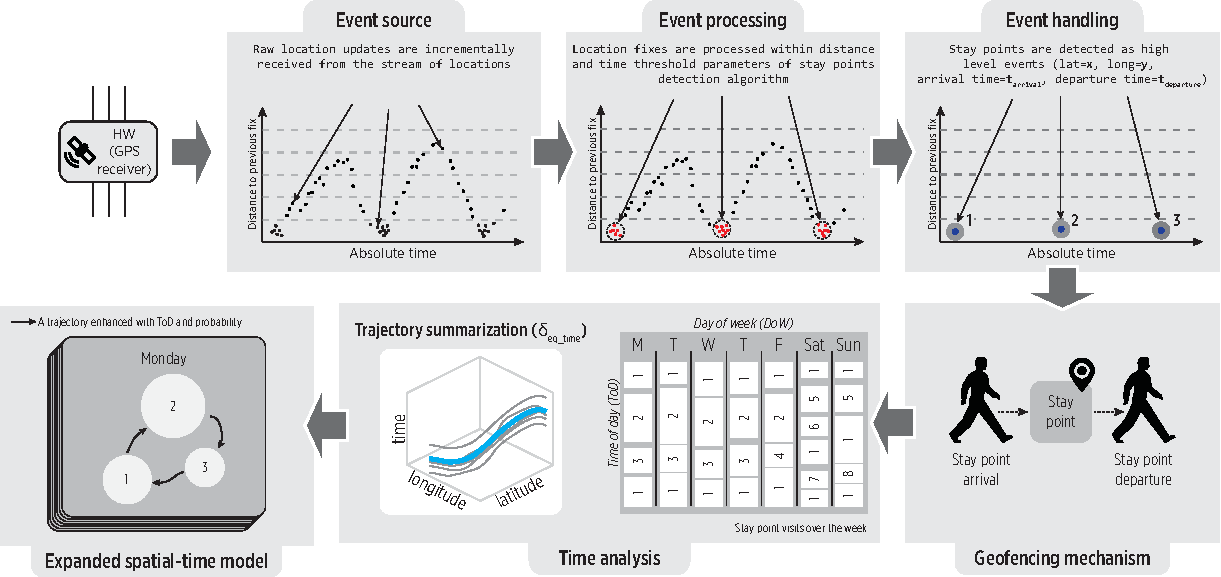
\includegraphics[width=\textwidth]{vectors/event-driven-memory-generation-for-slides}
  \captionof{figure}{A conceptual representation of the steps for generating the STM from raw sensors data.}
  \par
}
\end{block}
\end{frame}

\subsection{Working memory}
\begin{frame}{Working memory}{Probabilistic Reasoning Machine (PRM)}
\small
\begin{block}{\small \textbf{PRM features}}
\begin{itemize}
    \item It gives a meaning to the observed mobility information with respect of the STM information.
    \item It produces an estimation of future mobility state that links perceptual and working memory.
\end{itemize}
\end{block}

\begin{block}{\small \textbf{Interpretation}}
\begin{itemize}
  \item The \emph{Event Miner} traverses the STM for identifying whether learned information is:% (with respect of the STM):
  \begin{itemize}
     \item Consistent, or
     \item Inconsistent (mismatch)
   \end{itemize}
   with respect of observed mobility information.
\end{itemize}
\end{block}

\begin{block}{\small \textbf{Estimation}}
\begin{itemize}
\item The \emph{Event Miner} looks in the STM for a link (if any) with learned mobility information for generating spatial-time estimations:
\begin{itemize}
  \item Get next departure time.
  \item Get next arrival time.
\end{itemize}
\end{itemize}
\end{block}

\end{frame}

\subsection{Cognitive controller}
\begin{frame}{Cognitive controller (CC)}{Description}
\small
\vspace{-0.5cm}
\begin{columns}
\begin{column}[T]{0.5\textwidth}
\begin{block}{\small \textbf{Goals}}
  \begin{itemize}
      \item To reduce the energy consumption of location tracking by relying on PRM's estimations.
      \item To reduce the system uncertainty about current user mobility.
  \end{itemize}
\end{block}
\end{column}

\begin{column}[T]{0.5\textwidth}
\begin{block}{\small \textbf{Possible cognitive actions}}
  \begin{itemize}
    \item \textbf{Exploitation policies}: When system uncertainty is low for saving energy purposes.
    \item \textbf{Exploration policies}: When system uncertainty is high for recovering for accuracy loss.
  \end{itemize}
\end{block}
\end{column}
\end{columns}

\begin{figure}
  \centering
  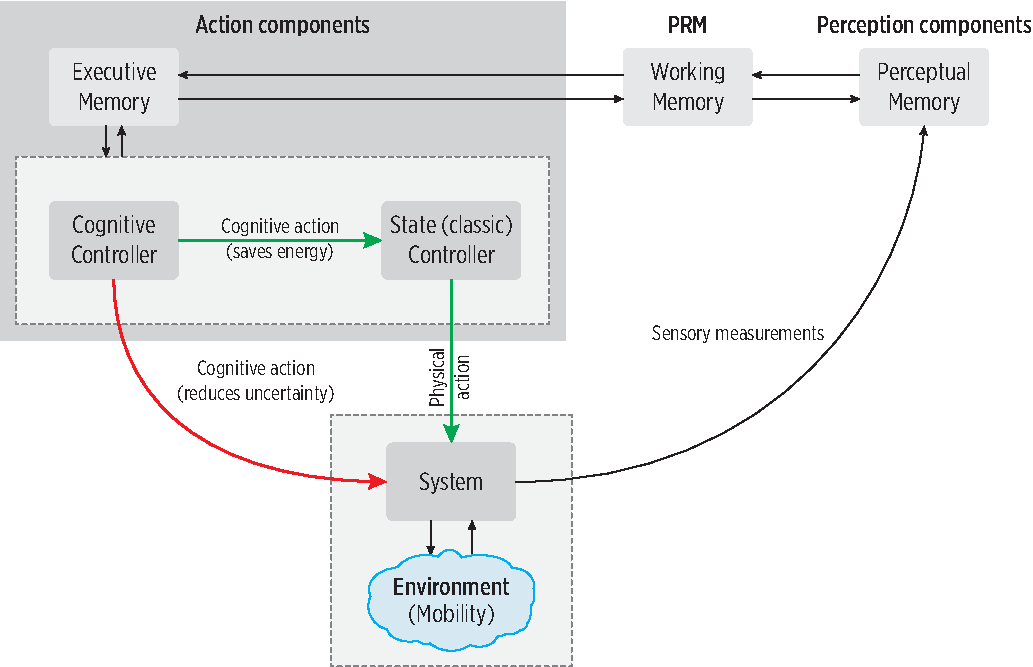
\includegraphics[width=0.65\textwidth]{vectors/cognitive-controller-architecture}
  \caption{A cognitive controller generic architecture}
\end{figure}

\end{frame}

\begin{frame}{Cognitive controller}{Policies tailored for user mobility}
\small
\begin{block}{\small \textbf{Stay point mode}}
  \begin{itemize}
      \item A sampling based on the sigmoid function $sig(x) = \frac{1}{1+e^{-\alpha x}}$ as a model for the mobility phase transitions.
      \item Higher sampling rate on arrival and departure, when the user is more likely to move, and slower at the middle of a visit.
      \item Central part is assisted by motion detection from the \emph{HAR} module.
  \end{itemize}
\end{block}

\begin{columns}
\begin{column}{0.45\textwidth}
\begin{figure}
  \centering
  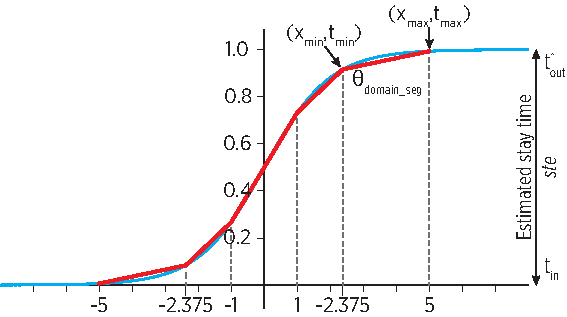
\includegraphics[width=0.99\linewidth]{vectors/sigmoid-segmentation-for-slides}
  \caption{Approximation of the sigmoid through straight segments.}
\end{figure}
\end{column}

\begin{column}{0.55\textwidth}
\begin{figure}
  \centering
  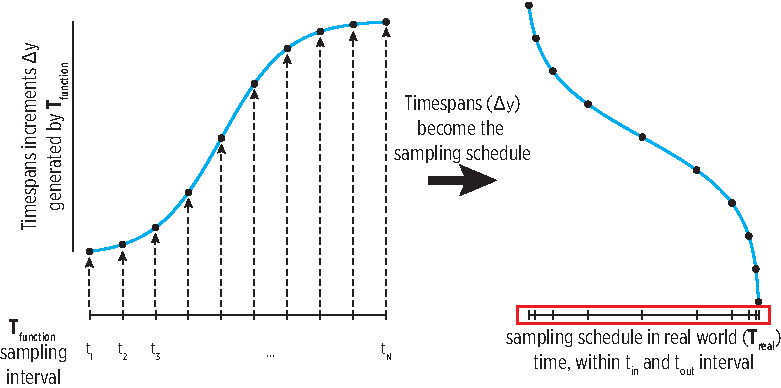
\includegraphics[width=0.99\linewidth]{vectors/sigmoid-driven-sampling-policy-for-slides}
  \caption{A snapshot of the process for producing a sigmoid sampling.}
\end{figure}
\end{column}
\end{columns}
\end{frame}

\begin{frame}{Cognitive controller}{Policies tailored for user mobility}
\small 
\begin{block}{\small \textbf{Trajectory mode}}
\begin{itemize}
    \item The spatiotemporal characterization of people's motion during trajectory is complex: it is hard to produce a single spatiotemporal model for summarizing how all people move.
    \item No special modeling of motion during a trajectory is performed other than the user moves within a speed range.
    \item A hint of such speed is provided by the HAR module from the detected transportation mode.
    \item The speed tendency over a window of identified transportation modes is employed for adjusting GPS sampling.
\end{itemize}
\end{block}

\begin{figure}
  \centering
  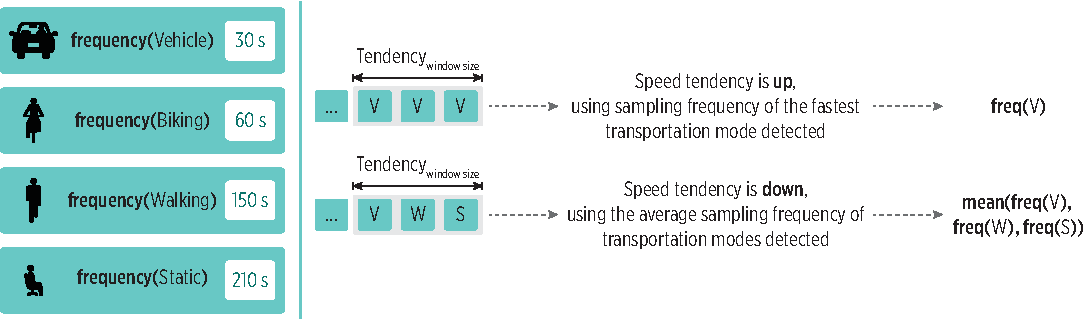
\includegraphics[width=0.7\linewidth]{vectors/trajectory-sampling.pdf}
  \caption{GPS sampling adaptation based on the speed tendency of detected transportation modes.}
\end{figure}
\end{frame}

\begin{frame}{Cognitive controller}{\emph{Sampling Decision Maker} module}
\small
\begin{block}{\small \textbf{Sampling Decision Maker module}}
  \begin{itemize}
      \item It filters from the \emph{pool of exploration-exploitation policies} those apt for the mobility state detected by PRM.
      \item It implements one policy, employing the spatial-time estimation provided by the PRM.
      \item It updates its \emph{Executive Memory} with the selected cognitive action for feedback in further executions.
  \end{itemize}
\end{block}

\begin{block}{\small \textbf{Reaction for mobility events}}
\begin{itemize}
  \item Reaction for arrival event:
  \begin{itemize}
  \item The sampling rate is reduced by following a sigmoid-based sampling.
  \end{itemize}

  \item Reaction for departure event:
  \begin{itemize}
    \item The sampling rate is increased by implementing a target sampling $T_{target}$.
  \end{itemize}
\end{itemize}
\end{block}
% {
%  \scriptsize 
% \begin{enumerate}
%   \item $\mathcal{T}_{function} = sigm_{t\_aware}(\Theta_{time\_sep},\Theta_{domain\_segs},t_{in},\hat{t_{out}})$
%   \item $\mathcal{T}_{real} = sampling\_generation(\mathcal{T}_{function}, t_{in},\hat{t_{out}}, func \shortleftarrow sigmoid)$ 
%   \item The reaction is expressed as: $\begin{aligned}[t]
%     CC_{arrival}(ste,m_{flag}\shortleftarrow false,\Theta_{time\_sep},&\Theta_{domain\_segs}) \\
%     &\rightarrow (GPS, \mathcal{T}_{real})
%   \end{aligned}$
% \end{enumerate}
% }

  % {
  % \scriptsize
  % \begin{enumerate}
  %   \item $\begin{aligned}[t]
  %   \mathcal{T}_{function} = linspace(t_{out},\hat{t_{in}}, \frac{\hat{t_{in}}-t_{out}}{T_{target}})
  %   \end{aligned}$

  %   \item $\mathcal{T}_{real} = sampling\_generation(\mathcal{T}_{function}, t_{out},\hat{t_{in}}, func \shortleftarrow x=y)$

  %   \item The reaction is expressed as: $CC_{departure}(ste,m_{flag}\shortleftarrow false, T_{target}) \rightarrow (GPS, \mathcal{T}_{real})$
    
  % \end{enumerate}
  % }
\end{frame}


\begin{frame}{Cognitive controller}{Mobility mismatches}
\small
\begin{block}{\small \textbf{Mismatches}}
  \begin{itemize}
    \item A mismatch represents a discrepancy between observed and learned mobility information.
    \item In general, the system increases the sampling rate for recovering the accuracy lost.
  \end{itemize}
\end{block}

\begin{block}{\small \textbf{Reaction for mobility mismatches}}
\begin{itemize}
  \item Reaction for early arrival:
  \begin{itemize}
    \item The sampling rate is reduced by following a sigmoid-based sampling.
  \end{itemize}

  \item Reaction for early departure:
  \begin{itemize}
    \item The fastest sampling rate is selected for recovering accuracy and improving system perception.
  \end{itemize}

  \item Reaction for late arrival:
  \begin{itemize}
    \item The fast sampling rate must be maintained as long as the user is still in trajectory.
  \end{itemize}

  \item Reaction for late departure:
  \begin{itemize}
    \item A \emph{conservative sampling} rate is implemented for detecting the eventual departure.
  \end{itemize}

\end{itemize}
\end{block}
\end{frame}
